La base de reglas se divide en dos partes principales:
\begin{itemize}
    \item \textbf{Parte deductiva}: Permite al agente inferir conocimiento nuevo o mejorar conocimiento previo mediante el uso de las percepciones captadas del entorno y la base de conocimiento.
    \item \textbf{Parte reactiva}: Permite al agente decidir que acción realizar en cada momento utilizando el conocimiento inferido.
\end{itemize}

Para simplificar las reglas, se utilizan los siguientes símbolos:
\begin{itemize}
    \item \textbf{S}: percepción de gemido.
    \item \textbf{A}: acción actual.
    \item $\mathbf{A^{t-1}}$: acción anterior.
    \item \textbf{H}: percepción de hedor.
    \item $\mathbf{W_{i, j}}$: monstruo en la casilla \emph{i, j}.
    \item $\mathbf{W?_{i, j}}$: posible monstruo en la casilla \emph{i, j}. 
    \item $\mathbf{OKW_{i, j}}$: no hay monstruo en la casilla \emph{i, j}. 
    \item $\mathbf{P_{i, j}}$: precipicio en la casilla \emph{i, j}.
    \item $\mathbf{P?_{i, j}}$: posible precipicio en la casilla \emph{i, j}. 
    \item $\mathbf{OKP_{i, j}}$: no hay precipicio en la casilla \emph{i, j}. 
    \item \textbf{R}: percepción de resplandor.
    \item $\mathbf{T_{i, j}}$: tesoro en la casilla \emph{i, j}.
    \item \textbf{G}: percepción de golpe.
    \item $\mathbf{M_{i, j}}$: muro en la casilla \emph{i, j}.
    \item $\mathbf{OK_{i, j}}$: casilla seguro (no contiene monstruos o precipicios)
    \item $\mathbf{V_{i, j}}$: casilla \emph{i, j} visitada.
    \item \textbf{PR}: número de proyectiles restantes.
    \item \textbf{BR}: número de bombas restantes.
    \item \textbf{CR}: número de ciclos restantes hasta lanzar la siguiente bomba.
    \item \textbf{SC}: número de casillas seguras que le queda al agente sin consumir.
\end{itemize}

\section{Parte deductiva}

Para simplificar la explicación, se han agrupado las reglas según las percepciones que recibe el agente.

Cuando un agente visita una casilla se le marca como visitada y se decrementa del número de casillas seguras conocidas sin visitar.

\begin{itemize}
    \item $\neg V_{i, j} \longrightarrow SC := SC - 1$
    \item $1 \longrightarrow V_{i, j}$
\end{itemize}

\centerline{\textbf{REGLAS DE CONSISTENCIA}}

Estas reglas sirven para garantizar la consistencia entre los estados de las casillas del mapa interno del agente. Estas reglas son:

\begin{itemize}
    \item $V_{i, j} \longrightarrow OK_{i, j}$
    \item $OK_{i, j} \iff OKW_{i, j} \land OKP_{i, j} $
    \item $OKW_{i, j} \longrightarrow \neg W?_{i, j} \land \neg W_{i, j} $
    \item $OKP_{i, j} \longrightarrow \neg P?_{i, j} \land \neg P_{i, j} $
    \item $P_{i, j} \longrightarrow \neg P?_{i, j} \land \neg W?_{i, j} \land \neg W_{i, j}$
    \item $W_{i, j} \longrightarrow \neg W?_{i, j} \land \neg P?_{i, j} \land \neg P_{i, j}$
    \item $W_{i, j} \longrightarrow \neg V_{i, j}$
\end{itemize}

\centerline{\textbf{GEMIDO}}

El gemido identifica la muerte de un monstruo. Este conocimiento es útil para el agente ya que indica que partes del entorno son seguras en el momento de oír el grito. Las reglas definen que:

\begin{itemize}
    \item Si el agente ha disparado en una dirección (al agente conoce la dirección en la que ha disparado) y ha oído un gemido, significa que la casilla adyacente es esa dirección es segura ya que si el monstruo estaba pegado al agente, habrá muerto y si no estaba pegado, la casilla era segura. Pero el gemido no dice nada respecto a las otras casillas, ya que pueden existir varios monstruos puestos en fila y un proyectil solo mataría al más cercano al agente.
    \item Si el agente ha disparado en una dirección y no oye un gemido, significa que en todas las casillas que siguen la dirección del disparo son seguras.
\end{itemize}

Las reglas que representan este conocimiento son (\emph{n} y \emph{m} son el ancho y alto del mapa respectivamente):
\begin{itemize}
    \item $ S \land A^{t-1} = DISPARAR\_NORTE \longrightarrow OKW_{i, j-1} $
    \item $ S \land A^{t-1} = DISPARAR\_ESTE \longrightarrow OKW_{i+1, j} $
    \item $ S \land A^{t-1} = DISPARAR\_SUR \longrightarrow OKW_{i, j+1} $
    \item $ S \land A^{t-1} = DISPARAR\_OESTE \longrightarrow OKW_{i-1, j} $
\end{itemize}

\begin{itemize}
    \item $ \neg S \land A^{t-1} = DISPARAR\_NORTE \longrightarrow OKW_{i, j-1} \land ... \land OKW_{i, 0} $
    \item $ \neg S \land A^{t-1} = DISPARAR\_ESTE \longrightarrow OKW_{i+1, j} \land ... \land OKW_{n-1, j}$
    \item $ \neg S \land A^{t-1} = DISPARAR\_SUR \longrightarrow OKW_{i, j+1}  \land ... \land OKW_{i, m-1}$
    \item $ \neg S \land A^{t-1} = DISPARAR\_OESTE \longrightarrow OKW_{i-1, j} \land ... \land OKW_{0, j}$ 
\end{itemize}

\centerline{\textbf{RESPLANDOR}}

La percepción de resplandor solo se puede captar sobre la casilla en la cual se encuentra una tesoro. Si no hay un resplandor en la casilla que se encuentra el agente, significa que no hay tesoro en esa casilla. Las reglas para inferir este conocimiento son:

\begin{itemize}
    \item $R_{i, j} \longrightarrow T_{i, j}$
    \item $\neg R_{i, j} \longrightarrow \neg T_{i, j}$
\end{itemize}

\centerline{\textbf{GOLPE}}

La percepción del golpe significa que el agente se ha golpeado con un muro. Ya que el agente sabe que el entorno es cuadrado, la acción que ha desencadenado el golpe y los muros solo delimitan la cueva del monstruo (mapa), cuando se da un golpe sabe que toda la fila o columna es son muros. Además, se descartan esas casillas del conjunto de casillas conocidas sin visitar. Las reglas para inferir este conocimiento son:

\begin{itemize}
    \item $G \land A^{t-1} = DESPLAZARSE\_NORTE \longrightarrow M_{0, j-1} \land ... \land M_{n, j-1}$
    \item $G \land A^{t-1} = DESPLAZARSE\_NORTE \land SC_{0, j-1} \longrightarrow SC := SC - 1,$ \newline
    $G \land A^{t-1} = DESPLAZARSE\_NORTE \land SC_{1, j-1} \longrightarrow SC := SC - 1,$ \newline
    $...,$ \newline
    $G \land A^{t-1} = DESPLAZARSE\_NORTE \land SC_{n, j-1} \longrightarrow SC := SC - 1$
    \item $G \land A^{t-1} = DESPLAZARSE\_ESTE \longrightarrow M_{i+1, 0} \land ... \land M_{i+1, m}$
    \item $G \land A^{t-1} = DESPLAZARSE\_ESTE \land SC_{i+1, 0} \longrightarrow SC := SC - 1,$ \newline
    $G \land A^{t-1} = DESPLAZARSE\_ESTE \land SC_{i+1, 1} \longrightarrow SC := SC - 1,$ \newline
    $...,$ \newline
    $G \land A^{t-1} = DESPLAZARSE\_ESTE \land SC_{i+1,m} \longrightarrow SC := SC - 1$
    \item $G \land A^{t-1} = DESPLAZARSE\_SUR \longrightarrow M_{0, j+1} \land ... \land M_{n, j+1}$
    \item $G \land A^{t-1} = DESPLAZARSE\_SUR \land SC_{0, j+1} \longrightarrow SC := SC - 1,$ \newline
    $G \land A^{t-1} = DESPLAZARSE\_SUR \land SC_{1, j+1} \longrightarrow SC := SC - 1,$ \newline
    $...,$ \newline
    $G \land A^{t-1} = DESPLAZARSE\_SUR \land SC_{n, j+1} \longrightarrow SC := SC - 1$
    \item $G \land A^{t-1} = DESPLAZARSE\_OESTE \longrightarrow M_{i-1, 0} \land ... \land M_{i-1, m}$
    \item $G \land A^{t-1} = DESPLAZARSE\_OESTE \land SC_{i-1, 0} \longrightarrow SC := SC - 1,$ \newline
    $G \land A^{t-1} = DESPLAZARSE\_OESTE \land SC_{i-1, 1} \longrightarrow SC := SC - 1,$ \newline
    $...,$ \newline
    $G \land A^{t-1} = DESPLAZARSE\_OESTE \land SC_{i-1,m} \longrightarrow SC := SC - 1$
\end{itemize}

\centerline{\textbf{HEDOR}}

La percepción del hedor avisa al agente de que existe un posible monstruo cerca. El agente sabe que solo puede existir un posible monstruo en las casillas adyacentes si estas no son muros o precipicios y si no han sido marcadas como visitadas o como que no puede haber monstruo en esa casilla. Las reglas para inferir este conocimiento son:

\begin{itemize}
    \item $H \land \neg M_{i, j-1} \land \neg P?_{i, j-1} \land \neg P_{i, j-1} \land \neg OKW_{i, j-1} \longrightarrow W?_{i, j-1}$
    \item $H \land \neg M_{i+1, j} \land \neg P?_{i+1, j} \land \neg P_{i+1, j} \land \neg OKW_{i+1, j} \longrightarrow W?_{i+1, j}$
    \item $H \land \neg M_{i, j+1} \land \neg P?_{i, j+1} \land \neg P_{i, j+1} \land \neg OKW_{i, j+1} \longrightarrow W?_{i, j+1}$
    \item $H \land \neg M_{i-1, j} \land \neg P?_{i-1, j} \land \neg P_{i-1, j} \land \neg OKW_{i-1, j} \longrightarrow W?_{i-1, j}$
\end{itemize}


Además, también sabe que si alguna las casillas adyacentes la había marcado como posible monstruo y cerca de esa casilla también hay otras dos casillas con hedores (en total 3 hedores), puede asegurar la existencia de un monstruo en la casilla marcada. Las reglas que permiten inferir este conocimiento son:

\begin{itemize}
    \item Se ha percibido el hedor al SUR de un posible monstruo (Figura 3.1 (a)):
        \begin{itemize}
             \item $H \land W?_{i, j-1} \land H_{i+1, j-1} \land H_{i, j-2} \longrightarrow W_{i, j-1}$
             \item $H \land W?_{i, j-1} \land H_{i+1, j-1} \land H_{i-1, j-1} \longrightarrow W_{i, j-1}$
             \item $H \land W?_{i, j-1} \land H_{i-1, j-1} \land H_{i, j-2} \longrightarrow W_{i, j-1}$
        \end{itemize}
        
    \item Se ha percibido el hedor al OESTE de un posible monstruo (Figura 3.1 (b)):
        \begin{itemize}
            \item $H \land W?_{i+1, j} \land H_{i+1, j+1} \land H_{i+2, j} \longrightarrow W_{i+1, j}$
            \item $H \land W?_{i+1, j} \land H_{i+1, j+1} \land H_{i+1, j-1} \longrightarrow W_{i+1, j}$
            \item $H \land W?_{i+1, j} \land H_{i-1, j-1} \land H_{i+2, j} \longrightarrow W_{i+1, j}$
        \end{itemize}
        
    \item Se ha percibido el hedor al NORTE de un posible monstruo (Figura 3.1 (c)):
        \begin{itemize}
           \item $H \land W?_{i, j+1} \land H_{i-1, j+1} \land H_{i, j+2} \longrightarrow W_{i, j+1}$
            \item $H \land W?_{i, j+1} \land H_{i-1, j+1} \land H_{i+1, j+1} \longrightarrow W_{i, j+1}$
            \item $H \land W?_{i, j+1} \land H_{i+1, j+1} \land H_{i, j+2} \longrightarrow W_{i, j+1}$
        \end{itemize}
        
    \item Se ha percibido el hedor al ESTE de un posible monstruo (Figura 3.1 (d)):
        \begin{itemize}
            \item $H \land W?_{i-1, j} \land H_{i-1, j-1} \land H_{i-2, j} \longrightarrow W_{i-1, j+1}$
            \item $H \land W?_{i-1, j} \land H_{i-1, j-1} \land H_{i-1, j+1} \longrightarrow W_{i-1, j+1}$
            \item $H \land W?_{i-1, j} \land H_{i-1, j+1} \land H_{i-2, j} \longrightarrow W_{i-1, j+1}$
        \end{itemize}
\end{itemize}

\begin{figure}[htb]
\centering
  \subfloat[W? al Norte]{%
    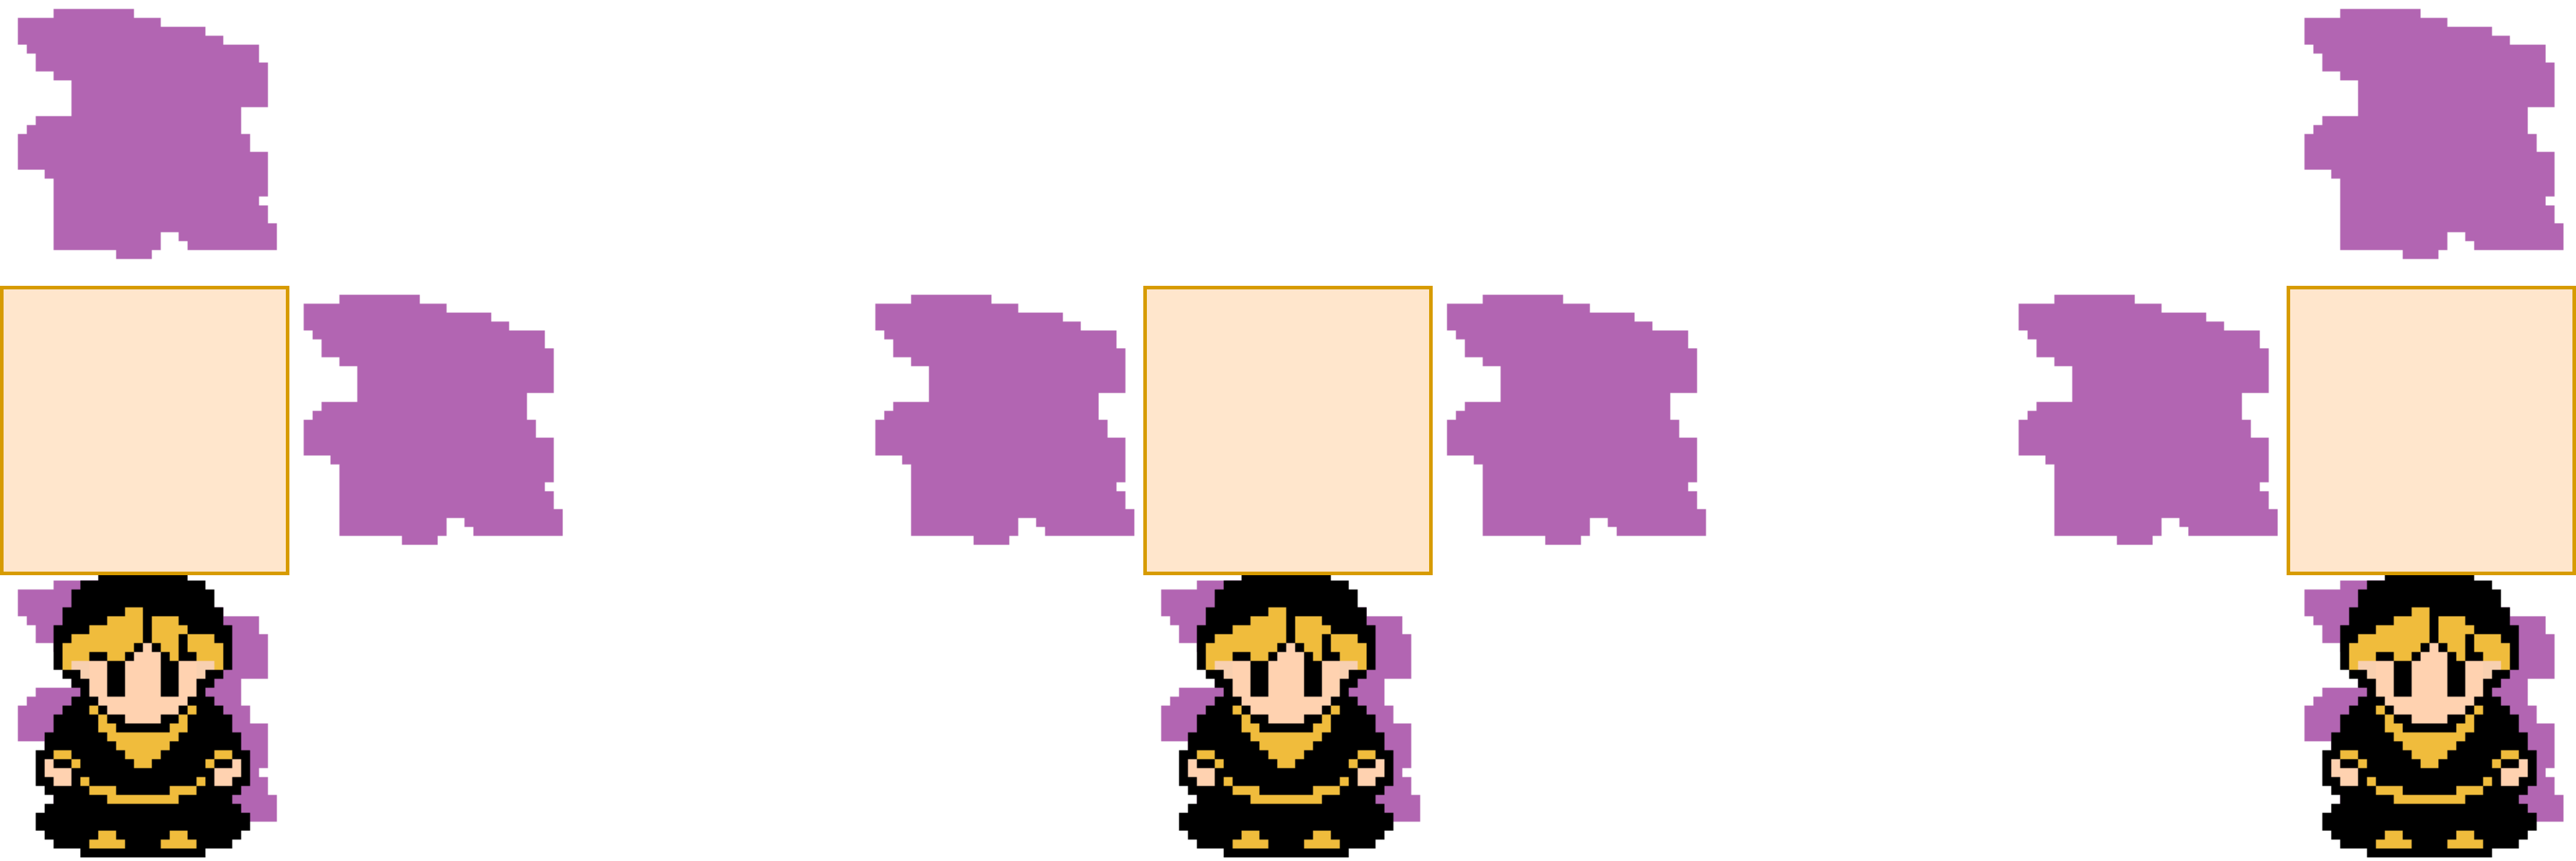
\includegraphics[width=.5\columnwidth]{w_norte}}\hspace{1em}
  \subfloat[W? al Este]{%
    
\includegraphics[width=.5\columnwidth]{w_este}}\\
  \subfloat[W? al Sur]{%
    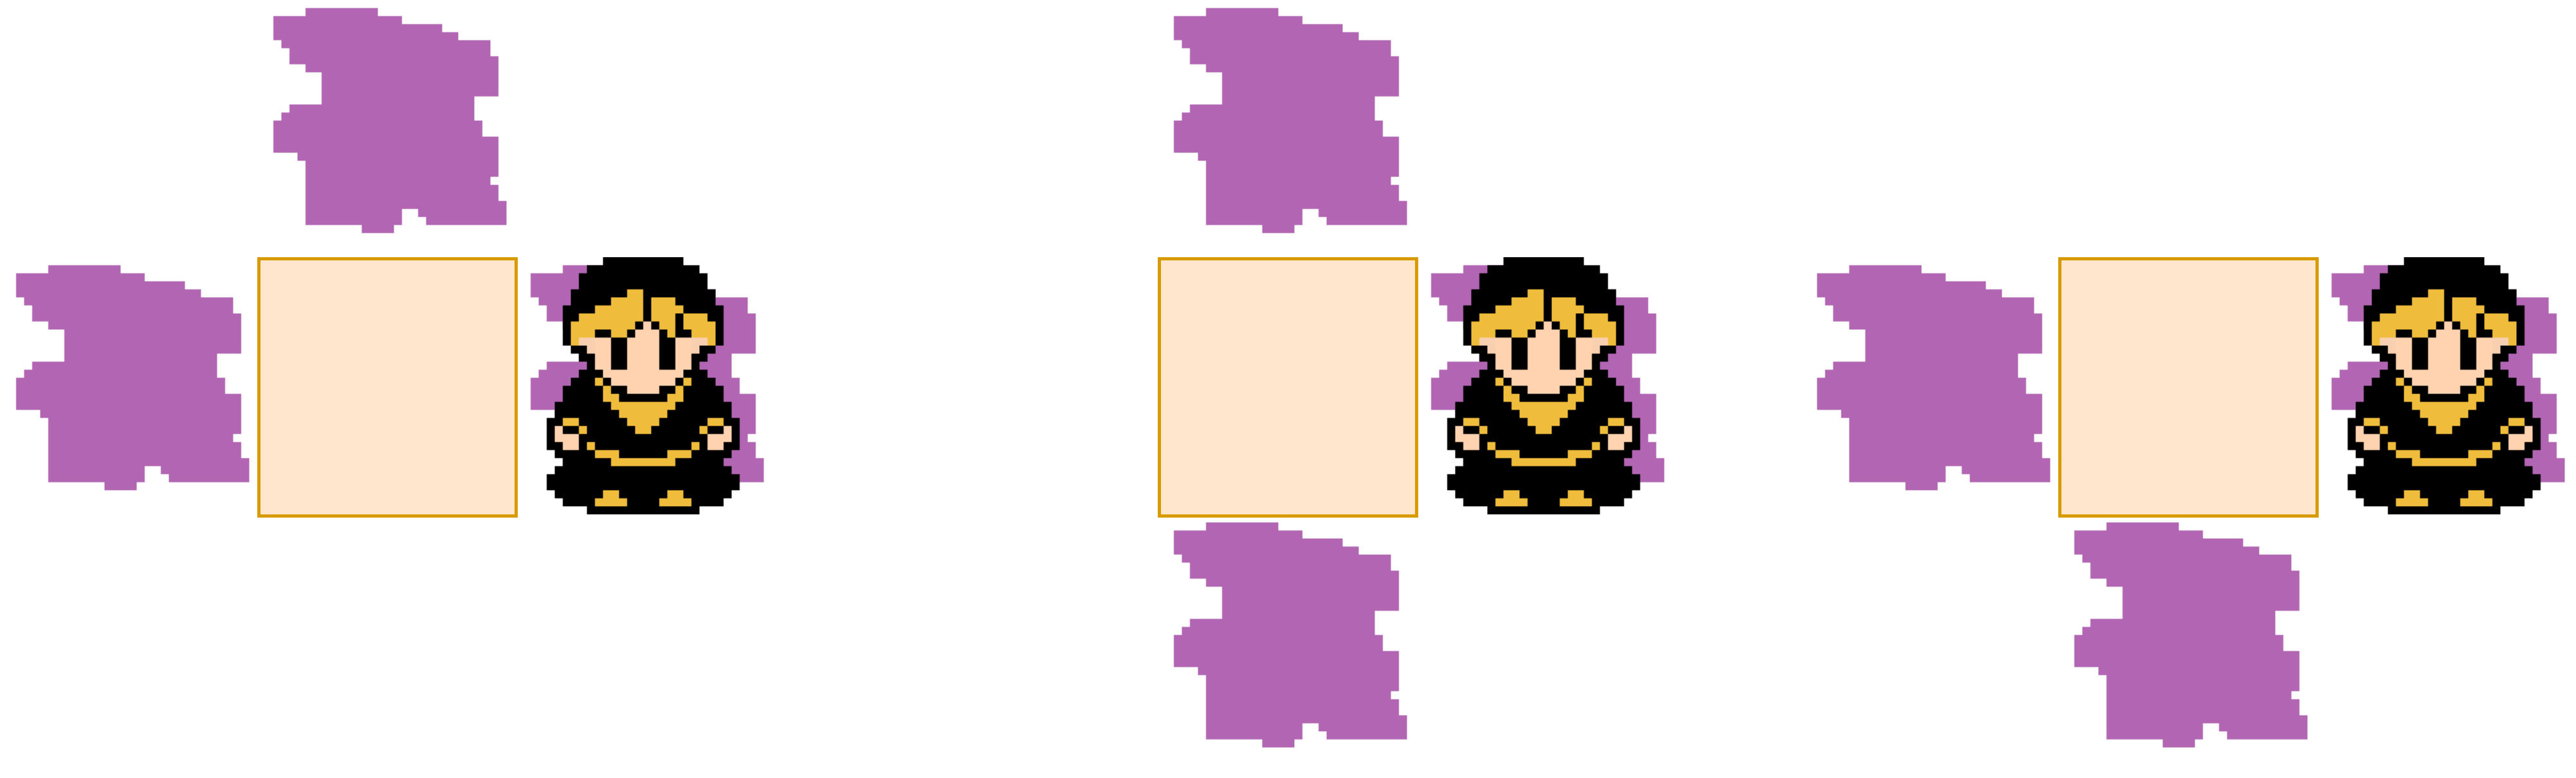
\includegraphics[width=.5\columnwidth]{w_sur}}\hspace{1em}
  \subfloat[W? al Oeste]{%
    
\includegraphics[width=.5\columnwidth]{w_oeste}}
  \caption{Inferir monstruo seguro}\label{fig:inferir_monstruo}
\end{figure}
\FloatBarrier

En caso de que no se haya percibido un hedor en la casilla en la que esta situado el agente, él sabe que las casillas adyacentes (\emph{Norte}, \emph{Este}, \emph{Sur} y \emph{Oeste}) es imposible que haya monstruos (los muros de la cueva no se pueden marcar como sin monstruo, ya que es incoherente hacerlo). Las reglas que permiten inferir esta conocimiento son:

\begin{itemize}
    \item $\neg H \land \neg M_{i, j-1} \longrightarrow OKW_{i, j-1}$
    \item $\neg H \land \neg M_{i+1, j} \longrightarrow OKW_{i+1, j}$
    \item $\neg H \land \neg M_{i, j+1} \longrightarrow OKW_{i, j+1}$
    \item $\neg H \land \neg M_{i-1, j1} \longrightarrow OKW_{i-1, j}$
\end{itemize}

\newpage
\centerline{\textbf{BRISA}}

La percepción de brisa indica que hay un posible precipicio cerca. El agente utiliza unas reglas similares a las de hedor para inferir sobre los precipicios (inferir posibles precipicios y precipicios seguros usando 3 brisas):

\begin{itemize}
    \item $B \land \neg M_{i, j-1} \land \neg W?_{i, j-1} \land \neg W_{i, j-1} \land \neg OKP_{i, j-1} \longrightarrow P?_{i, j-1}$
    \item $B \land \neg M_{i+1, j} \land \neg W?_{i+1, j} \land \neg W_{i+1, j} \land \neg OKP_{i+1, j} \longrightarrow P?_{i+1, j}$
    \item $B \land \neg M_{i, j+1} \land \neg W?_{i, j+1} \land \neg W_{i, j+1} \land \neg OKP_{i, j+1} \longrightarrow P?_{i, j+1}$
    \item $B \land \neg M_{i-1, j} \land \neg W?_{i-1, j} \land \neg W_{i-1, j} \land \neg OKP_{i-1, j} \longrightarrow P?_{i-1, j}$
\end{itemize}

\begin{itemize}
    \item Se ha percibido la brisa al SUR de un posible monstruo (Figura 3.2 (a)):
        \begin{itemize}
             \item $B \land P?_{i, j-1} \land B_{i+1, j-1} \land B_{i, j-2} \longrightarrow P_{i, j-1}$
             \item $B \land P?_{i, j-1} \land B_{i+1, j-1} \land B_{i-1, j-1} \longrightarrow P_{i, j-1}$
             \item $B \land P?_{i, j-1} \land B_{i-1, j-1} \land B_{i, j-2} \longrightarrow P_{i, j-1}$
        \end{itemize}
        
    \item Se ha percibido la brisa al OESTE de un posible monstruo (Figura 3.2 (b)):
        \begin{itemize}
            \item $B \land P?_{i+1, j} \land B_{i+1, j+1} \land B_{i+2, j} \longrightarrow P_{i+1, j}$
            \item $B \land P?_{i+1, j} \land B_{i+1, j+1} \land B_{i+1, j-1} \longrightarrow P_{i+1, j}$
            \item $B \land P?_{i+1, j} \land B_{i-1, j-1} \land B_{i+2, j} \longrightarrow P_{i+1, j}$
        \end{itemize}
        
    \item Se ha percibido la brisa al NORTE de un posible monstruo (Figura 3.2 (c)):
        \begin{itemize}
           \item $B \land P?_{i, j+1} \land B_{i-1, j+1} \land B_{i, j+2} \longrightarrow P_{i, j+1}$
            \item $B \land P?_{i, j+1} \land B_{i-1, j+1} \land B_{i+1, j+1} \longrightarrow P_{i, j+1}$
            \item $B \land P?_{i, j+1} \land B_{i+1, j+1} \land B_{i, j+2} \longrightarrow P_{i, j+1}$
        \end{itemize}
        
    \item Se ha percibido la brisa al ESTE de un posible monstruo (Figura 3.2 (d)):
        \begin{itemize}
            \item $B \land P?_{i-1, j} \land B_{i-1, j-1} \land B_{i-2, j} \longrightarrow P_{i-1, j+1}$
            \item $B \land P?_{i-1, j} \land B_{i-1, j-1} \land B_{i-1, j+1} \longrightarrow P_{i-1, j+1}$
            \item $B \land P?_{i-1, j} \land B_{i-1, j+1} \land B_{i-2, j} \longrightarrow P_{i-1, j+1}$
        \end{itemize}
\end{itemize}

\begin{figure}[htb]
\centering
  \subfloat[P? al Norte]{%
    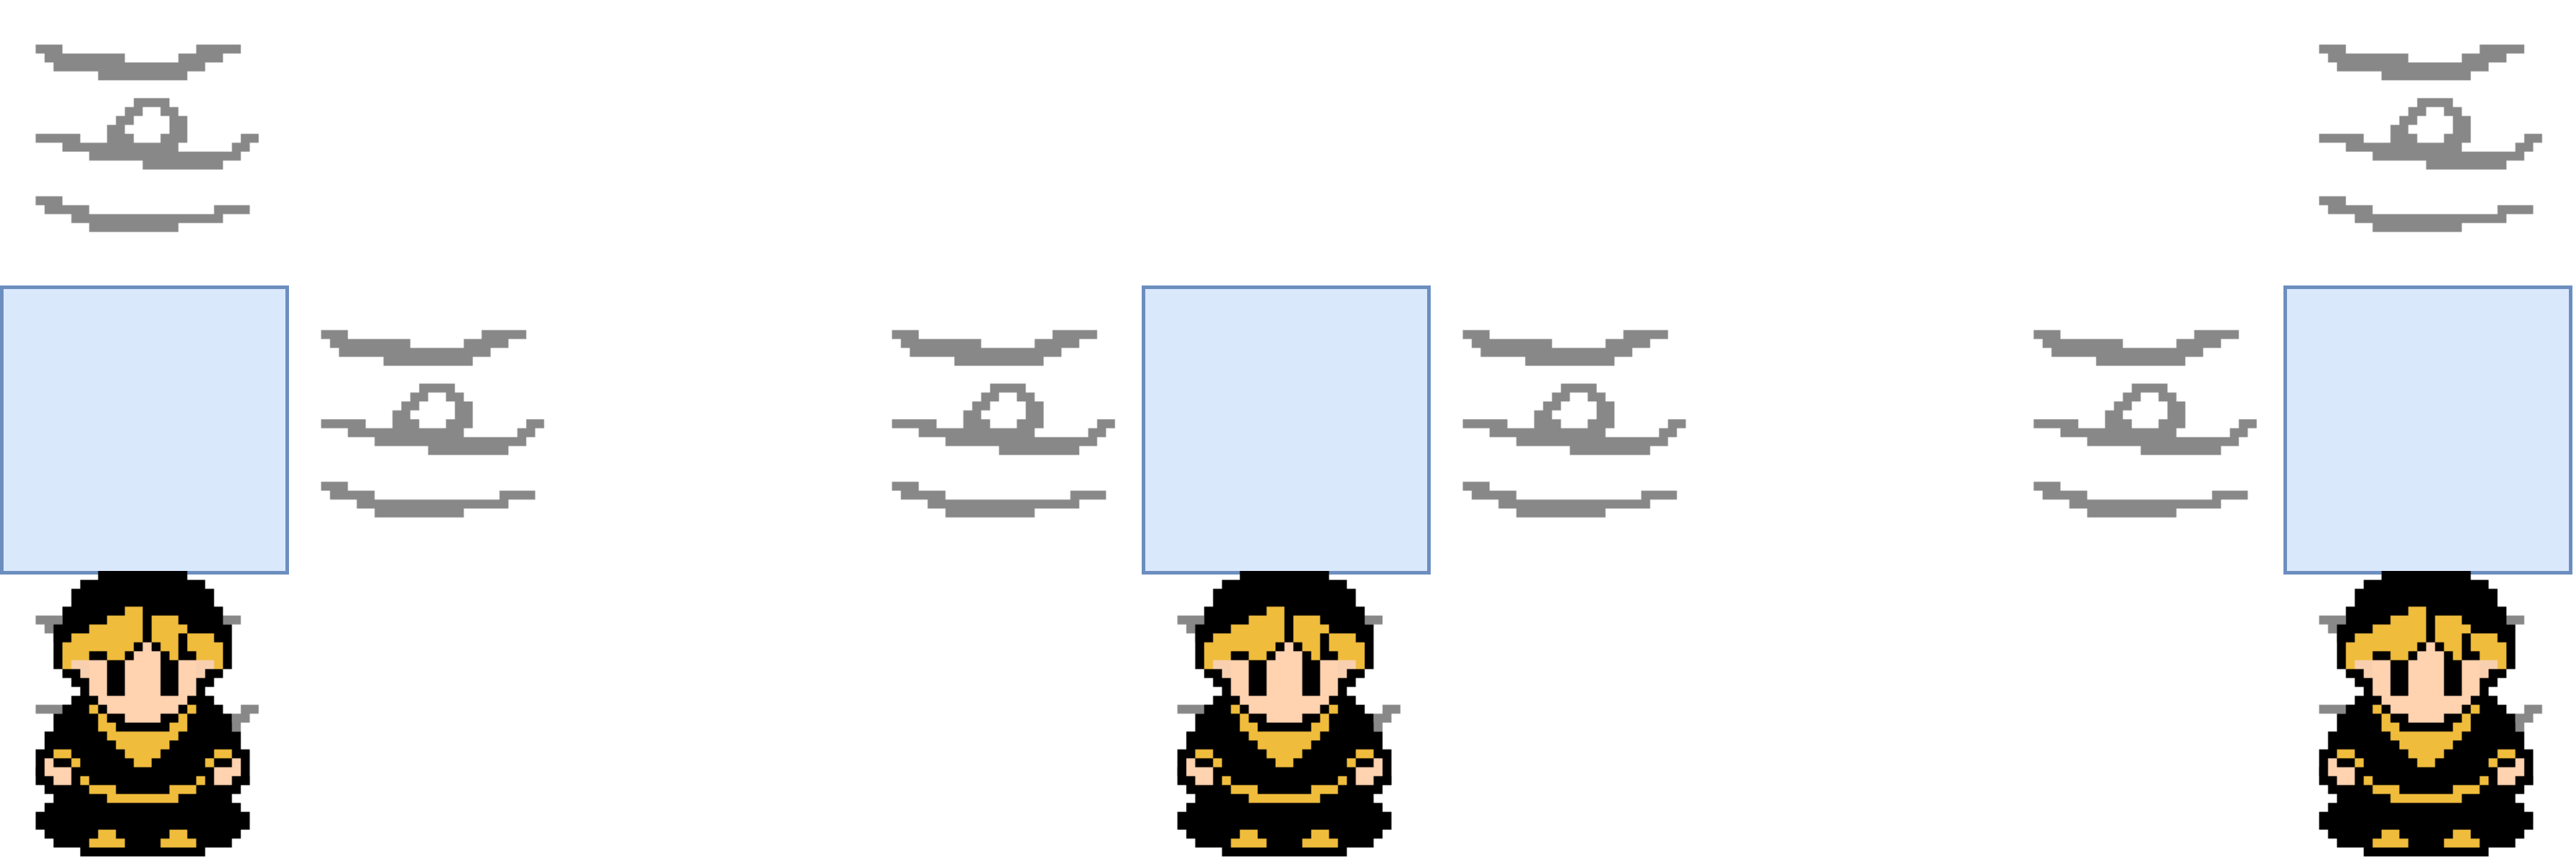
\includegraphics[width=.5\columnwidth]{p_norte}}\hspace{1em}
  \subfloat[P? al Este]{%
    
\includegraphics[width=.5\columnwidth]{p_este}}\\
  \subfloat[P? al Sur]{%
    
\includegraphics[width=.5\columnwidth]{p_sur}}\hspace{1em}
  \subfloat[P? al Oeste]{%
    
\includegraphics[width=.5\columnwidth]{p_oeste}}
  \caption{Inferir precipicio seguro}\label{fig:inferir_precipicio}
\end{figure}
\FloatBarrier

\begin{itemize}
    \item $\neg B \land \neg M_{i, j-1} \longrightarrow OKP_{i, j-1}$
    \item $\neg B \land \neg M_{i+1, j} \longrightarrow OKP_{i+1, j}$
    \item $\neg B \land \neg M_{i, j+1} \longrightarrow OKP_{i, j+1}$
    \item $\neg B \land \neg M_{i-1, j1} \longrightarrow OKP_{i-1, j}$
\end{itemize}

\centerline{\textbf{INCREMENTAR CASILLAS SEGURAS SIN CONSUMIR}}

Se incrementa el contador de casillas seguras conocidas sin visitar en función del número de casillas seguras adyacentes sin visitar y se las marca como sin consumir.

\begin{itemize}
    \item $OK_{i, j-1} \wedge \neg V_{i,j-1} \wedge \neg SC_{i, j-1} \longrightarrow SC := SC + 1, SC_{i,j-1}$
    \item $OK_{i+1, j} \wedge \neg V_{i+1,j} \wedge \neg SC_{i+1, j} \longrightarrow SC := SC + 1, SC_{i+1,j}$
    \item $OK_{i, j+1} \wedge \neg V_{i,j+1} \wedge \neg SC_{i, j+1} \longrightarrow SC := SC + 1, SC_{i,j+1}$
    \item $OK_{i-1, j} \wedge \neg V_{i-1,j} \wedge \neg SC_{i-1, j} \longrightarrow SC := SC + 1, SC_{i-1,j}$
\end{itemize}

\section{Parte reactiva}

En la parte reactiva de las reglas que permiten realizar acciones correctas y seguras con el conocimiento inferido en la base de conocimientos. Estas reglas son:

\begin{itemize}
    \item Recoger el tesoro en una casillas con resplandor.
        \begin{itemize}
            \item   $X_1 \longrightarrow RECOGER\_TESORO \equiv$
                    \newline
                    $T_{i, j} \longrightarrow RECOGER\_TESORO$
        \end{itemize}
        
    \item Lanzar bombas de hedor cuando el tiempo de espera (aleatorio) ha terminado.
        \begin{itemize}
            \item $X_2 \longrightarrow PRODUCIR\_HEDOR$
            \newline
            $CR = 0 \land BR > 0 \longrightarrow PRODUCIR\_HEDOR$
        \end{itemize}
    
    \item Matar el monstruo seguro (se prefiere a visitar casillas adyacentes que la muerte de un monstruo puede suponer la posibilidad de explorar más la cueva y encontrar el tesoro): 
        \begin{itemize}
            \item   $X_3 \longrightarrow DISPARAR\_NORTE \equiv$
                    \newline
                    $W_{i, j-1} \land PR > 0 \longrightarrow DISPARAR\_NORTE$
            \item   $X_4 \longrightarrow DISPARAR\_ESTE \equiv$
                    \newline
                    $W_{i+1, j} \land PR > 0 \longrightarrow DISPARAR\_ESTE$
            \item   $X_5 \longrightarrow DISPARAR\_SUR \equiv$
                    \newline
                    $W_{i, j+1} \land PR > 0 \longrightarrow DISPARAR\_SUR$
            \item   $X_6 \longrightarrow DISPARAR\_OESTE \equiv$
                    \newline
                    $W_{i-1, j} \land PR > 0 \longrightarrow DISPARAR\_OESTE$
        \end{itemize}
    
    \item Explorar casillas no visitadas y que sean seguras:
        \begin{itemize}
            \item   $ X_7                 \longrightarrow$
                    $A = DESPLAZARSE\_NORTE $
                    $\equiv$
                    \newline
                    $ A = NINGUNA \land \neg M_{i, j-1} \land \neg V_{i, j-1} \land OK_{i, j-1} \longrightarrow$
                    \newline
                    $A = DESPLAZARSE\_NORTE$
            
             \item  $ X_8                 \longrightarrow$
                    $A = DESPLAZARSE\_ESTE $
                    $\equiv$
                    \newline
                    $ A = NINGUNA \land \neg M_{i+1, j} \land \neg V_{i+1, j} \land OK_{i+1, j} \longrightarrow$
                    \newline
                    $A = DESPLAZARSE\_ESTE $
                    
             \item  $ X_9                 \longrightarrow$
                    $A = DESPLAZARSE\_SUR $
                    $\equiv$
                    \newline
                    $ A = NINGUNA \land \neg M_{i, j+1} \land \neg V_{i, +1j} \land OK_{i, j+1} \longrightarrow$
                    \newline
                    $A = DESPLAZARSE\_SUR $
            
             \item  $ X_{10}                 \longrightarrow$
                    $A = DESPLAZARSE\_OESTE $
                    $\equiv$
                    \newline
                    $ A = NINGUNA \land \neg M_{i-1, j} \land \neg V_{i-1, j} \land OK_{i-1, j} \longrightarrow$
                    \newline
                    $A = DESPLAZARSE\_OESTE $
            
        \end{itemize}
    
    \item Realizar un disparo en caso de que existan posibles monstruos y el agente no tenga más casillas por explorar:
        \begin{itemize}
            \item $X_{11} \longrightarrow DISPARAR\_NORTE$
            $\equiv$
            \newline
            $A = NINGUNA \land SC = 0 \land W?_{i, j-1} \land PR > 0$ 
            
            $\longrightarrow DISPARAR\_NORTE$
            
            \item $X_{12} \longrightarrow DISPARAR\_ESTE$
            $\equiv$
            \newline
            $A = NINGUNA \land SC = 0 \land W?_{i+1, j} \land PR > 0$ 
            
            $\longrightarrow DISPARAR\_ESTE$
            
            \item $X_{13} \longrightarrow DISPARAR\_SUR$
            $\equiv$
            \newline
            $A = NINGUNA \land SC = 0 \land W?_{i, j+1} \land PR > 0$ 
            
            $\longrightarrow DISPARAR\_SUR$
            
            \item $X_{14} \longrightarrow DISPARAR\_OESTE$
            $\equiv$
            \newline
            $A = NINGUNA \land SC = 0 \land W?_{i-1, j} \land PR > 0$ 
            
            $\longrightarrow DISPARAR\_OESTE$
        \end{itemize}
    
    \item Volver a la casilla anterior (realizar la acción contraria) en caso de que no se haya podido cumplir ninguno de los casos anteriores:
        \begin{itemize}
            \item $A = NINGUNA \longrightarrow VOLVER\_CASILLA\_ANTERIOR$
        \end{itemize}
\end{itemize}

\newpage
\section{Todas las reglas}

Finalmente, el conjunto de todas las reglas es:
\begin{enumerate}
    \item $\neg V_{i, j} \longrightarrow SC := SC - 1$
    \item $1 \longrightarrow V_{i, j}$
    \item $V_{i, j} \longrightarrow OK_{i, j}$
    \item $OK_{i, j} \iff OKW_{i, j} \land OKP_{i, j} $
    \item $OKW_{i, j} \longrightarrow \neg W?_{i, j} \land \neg W_{i, j} $
    \item $OKP_{i, j} \longrightarrow \neg P?_{i, j} \land \neg P_{i, j} $
    \item $P_{i, j} \longrightarrow \neg P?_{i, j} \land \neg W?_{i, j} \land \neg W_{i, j}$
    \item $W_{i, j} \longrightarrow \neg W?_{i, j} \land \neg P?_{i, j} \land \neg P_{i, j}$
    \item $W_{i, j} \longrightarrow \neg V_{i, j}$
    \item $ S \land A^{t-1} = DISPARAR\_NORTE \longrightarrow OKW_{i, j-1} $
    \item $ S \land A^{t-1} = DISPARAR\_ESTE \longrightarrow OKW_{i+1, j} $
    \item $ S \land A^{t-1} = DISPARAR\_SUR \longrightarrow OKW_{i, j+1} $
    \item $ S \land A^{t-1} = DISPARAR\_OESTE \longrightarrow OKW_{i-1, j} $
    \item $ \neg S \land A^{t-1} = DISPARAR\_NORTE \longrightarrow OKW_{i, j-1} \land ... \land OKW_{i, 0} $
    \item $ \neg S \land A^{t-1} = DISPARAR\_ESTE \longrightarrow OKW_{i+1, j} \land ... \land OKW_{n-1, j}$
    \item $ \neg S \land A^{t-1} = DISPARAR\_SUR \longrightarrow OKW_{i, j+1}  \land ... \land OKW_{i, m-1}$
    \item $ \neg S \land A^{t-1} = DISPARAR\_OESTE \longrightarrow OKW_{i-1, j} \land ... \land OKW_{0, j}$ 
    \item $R_{i, j} \longrightarrow T_{i, j}$
    \item $\neg R_{i, j} \longrightarrow \neg T_{i, j}$
    \item $G \land A^{t-1} = DESPLAZARSE\_NORTE \longrightarrow M_{0, j-1} \land ... \land M_{n, j-1}$
    \item $G \land A^{t-1} = DESPLAZARSE\_NORTE \land SC_{0, j-1} \longrightarrow SC := SC - 1,$ \newline
    $G \land A^{t-1} = DESPLAZARSE\_NORTE \land SC_{1, j-1} \longrightarrow SC := SC - 1,$ \newline
    $...,$ \newline
    $G \land A^{t-1} = DESPLAZARSE\_NORTE \land SC_{n, j-1} \longrightarrow SC := SC - 1$
    \item $G \land A^{t-1} = DESPLAZARSE\_ESTE \longrightarrow M_{i+1, 0} \land ... \land M_{i+1, m}$
    \item $G \land A^{t-1} = DESPLAZARSE\_ESTE \land SC_{i+1, 0} \longrightarrow SC := SC - 1,$ \newline
    $G \land A^{t-1} = DESPLAZARSE\_ESTE \land SC_{i+1, 1} \longrightarrow SC := SC - 1,$ \newline
    $...,$ \newline
    $G \land A^{t-1} = DESPLAZARSE\_ESTE \land SC_{i+1,m} \longrightarrow SC := SC - 1$
    \item $G \land A^{t-1} = DESPLAZARSE\_SUR \longrightarrow M_{0, j+1} \land ... \land M_{n, j+1}$
    \item $G \land A^{t-1} = DESPLAZARSE\_SUR \land SC_{0, j+1} \longrightarrow SC := SC - 1,$ \newline
    $G \land A^{t-1} = DESPLAZARSE\_SUR \land SC_{1, j+1} \longrightarrow SC := SC - 1,$ \newline
    $...,$ \newline
    $G \land A^{t-1} = DESPLAZARSE\_SUR \land SC_{n, j+1} \longrightarrow SC := SC - 1$
    \item $G \land A^{t-1} = DESPLAZARSE\_OESTE \longrightarrow M_{i-1, 0} \land ... \land M_{i-1, m}$
    \item $G \land A^{t-1} = DESPLAZARSE\_OESTE \land SC_{i-1, 0} \longrightarrow SC := SC - 1,$ \newline
    $G \land A^{t-1} = DESPLAZARSE\_OESTE \land SC_{i-1, 1} \longrightarrow SC := SC - 1,$ \newline
    $...,$ \newline
    $G \land A^{t-1} = DESPLAZARSE\_OESTE \land SC_{i-1,m} \longrightarrow SC := SC - 1$
    \item $H \land \neg M_{i, j-1} \land \neg P?_{i, j-1} \land \neg P_{i, j-1} \land \neg OKW_{i, j-1} \longrightarrow W?_{i, j-1}$
    \item $H \land \neg M_{i+1, j} \land \neg P?_{i+1, j} \land \neg P_{i+1, j} \land \neg OKW_{i+1, j} \longrightarrow W?_{i+1, j}$
    \item $H \land \neg M_{i, j+1} \land \neg P?_{i, j+1} \land \neg P_{i, j+1} \land \neg OKW_{i, j+1} \longrightarrow W?_{i, j+1}$
    \item $H \land \neg M_{i-1, j} \land \neg P?_{i-1, j} \land \neg P_{i-1, j} \land \neg OKW_{i-1, j} \longrightarrow W?_{i-1, j}$
    \item $H \land W?_{i, j-1} \land H_{i+1, j-1} \land H_{i, j-2} \longrightarrow W_{i, j-1}$
    \item $H \land W?_{i, j-1} \land H_{i+1, j-1} \land H_{i-1, j-1} \longrightarrow W_{i, j-1}$
    \item $H \land W?_{i, j-1} \land H_{i-1, j-1} \land H_{i, j-2} \longrightarrow W_{i, j-1}$
    
    \item $H \land W?_{i+1, j} \land H_{i+1, j+1} \land H_{i+2, j} \longrightarrow W_{i+1, j}$
    \item $H \land W?_{i+1, j} \land H_{i+1, j+1} \land H_{i+1, j-1} \longrightarrow W_{i+1, j}$
    \item $H \land W?_{i+1, j} \land H_{i-1, j-1} \land H_{i+2, j} \longrightarrow W_{i+1, j}$
    
    \item $H \land W?_{i, j+1} \land H_{i-1, j+1} \land H_{i, j+2} \longrightarrow W_{i, j+1}$
    \item $H \land W?_{i, j+1} \land H_{i-1, j+1} \land H_{i+1, j+1} \longrightarrow W_{i, j+1}$
    \item $H \land W?_{i, j+1} \land H_{i+1, j+1} \land H_{i, j+2} \longrightarrow W_{i, j+1}$
    
    \item $H \land W?_{i-1, j} \land H_{i-1, j-1} \land H_{i-2, j} \longrightarrow W_{i-1, j+1}$
    \item $H \land W?_{i-1, j} \land H_{i-1, j-1} \land H_{i-1, j+1} \longrightarrow W_{i-1, j+1}$
    \item $H \land W?_{i-1, j} \land H_{i-1, j+1} \land H_{i-2, j} \longrightarrow W_{i-1, j+1}$
    
    \item $B \land \neg M_{i, j-1} \land \neg W?_{i, j-1} \land \neg W_{i, j-1} \land \neg OKP_{i, j-1} \longrightarrow P?_{i, j-1}$
    \item $B \land \neg M_{i+1, j} \land \neg W?_{i+1, j} \land \neg W_{i+1, j} \land \neg OKP_{i+1, j} \longrightarrow P?_{i+1, j}$
    \item $B \land \neg M_{i, j+1} \land \neg W?_{i, j+1} \land \neg W_{i, j+1} \land \neg OKP_{i, j+1} \longrightarrow P?_{i, j+1}$
    \item $B \land \neg M_{i-1, j} \land \neg W?_{i-1, j} \land \neg W_{i-1, j} \land \neg OKP_{i-1, j} \longrightarrow P?_{i-1, j}$
    \item $B \land P?_{i, j-1} \land B_{i+1, j-1} \land B_{i, j-2} \longrightarrow P_{i, j-1}$
    \item $B \land P?_{i, j-1} \land B_{i+1, j-1} \land B_{i-1, j-1} \longrightarrow P_{i, j-1}$
    \item $B \land P?_{i, j-1} \land B_{i-1, j-1} \land B_{i, j-2} \longrightarrow P_{i, j-1}$
    
    \item $B \land P?_{i+1, j} \land B_{i+1, j+1} \land B_{i+2, j} \longrightarrow P_{i+1, j}$
    \item $B \land P?_{i+1, j} \land B_{i+1, j+1} \land B_{i+1, j-1} \longrightarrow P_{i+1, j}$
    \item $B \land P?_{i+1, j} \land B_{i-1, j-1} \land B_{i+2, j} \longrightarrow P_{i+1, j}$
    
    \item $B \land P?_{i, j+1} \land B_{i-1, j+1} \land B_{i, j+2} \longrightarrow P_{i, j+1}$
    \item $B \land P?_{i, j+1} \land B_{i-1, j+1} \land B_{i+1, j+1} \longrightarrow P_{i, j+1}$
    \item $B \land P?_{i, j+1} \land B_{i+1, j+1} \land B_{i, j+2} \longrightarrow P_{i, j+1}$
    
    \item $B \land P?_{i-1, j} \land B_{i-1, j-1} \land B_{i-2, j} \longrightarrow P_{i-1, j+1}$
    \item $B \land P?_{i-1, j} \land B_{i-1, j-1} \land B_{i-1, j+1} \longrightarrow P_{i-1, j+1}$
    \item $B \land P?_{i-1, j} \land B_{i-1, j+1} \land B_{i-2, j} \longrightarrow P_{i-1, j+1}$
    
    \item $OK_{i, j-1} \wedge \neg V_{i,j-1} \wedge \neg SC_{i, j-1} \longrightarrow SC := SC + 1, SC_{i,j-1}$
    \item $OK_{i+1, j} \wedge \neg V_{i+1,j} \wedge \neg SC_{i+1, j} \longrightarrow SC := SC + 1, SC_{i+1,j}$
    \item $OK_{i, j+1} \wedge \neg V_{i,j+1} \wedge \neg SC_{i, j+1} \longrightarrow SC := SC + 1, SC_{i,j+1}$
    \item $OK_{i-1, j} \wedge \neg V_{i-1,j} \wedge \neg SC_{i-1, j} \longrightarrow SC := SC + 1, SC_{i-1,j}$
\newline
    \item   $X_1 \longrightarrow RECOGER\_TESORO \equiv$
    \newline
    $T_{i, j} \longrightarrow RECOGER\_TESORO$

    \item $X_2 \longrightarrow PRODUCIR\_HEDOR$
    \newline
    $CR = 0 \land BR > 0 \longrightarrow PRODUCIR\_HEDOR$

    \item   $X_3 \longrightarrow DISPARAR\_NORTE \equiv$
    \newline
    $W_{i, j-1} \land PR > 0 \longrightarrow DISPARAR\_NORTE$

    \item   $X_4 \longrightarrow DISPARAR\_ESTE \equiv$
    \newline
    $W_{i+1, j} \land PR > 0 \longrightarrow DISPARAR\_ESTE$

    \item   $X_5 \longrightarrow DISPARAR\_SUR \equiv$
    \newline
    $W_{i, j+1} \land PR > 0 \longrightarrow DISPARAR\_SUR$

    \item   $X_6 \longrightarrow DISPARAR\_OESTE \equiv$
    \newline
    $W_{i-1, j} \land PR > 0 \longrightarrow DISPARAR\_OESTE$

    \item   $ X_7                 \longrightarrow$
    $A = DESPLAZARSE\_NORTE $
    $\equiv$
    \newline
    $ A = NINGUNA \land \neg M_{i, j-1} \land \neg V_{i, j-1} \land OK_{i, j-1} \longrightarrow$
    \newline
    $A = DESPLAZARSE\_NORTE$
            
    \item  $ X_8                 \longrightarrow$
    $A = DESPLAZARSE\_ESTE $
    $\equiv$
    \newline
    $ A = NINGUNA \land \neg M_{i+1, j} \land \neg V_{i+1, j} \land OK_{i+1, j} \longrightarrow$
    \newline
    $A = DESPLAZARSE\_ESTE $
                    
    \item  $ X_9                 \longrightarrow$
    $A = DESPLAZARSE\_SUR $
    $\equiv$
    \newline
    $ A = NINGUNA \land \neg M_{i, j+1} \land \neg V_{i, +1j} \land OK_{i, j+1} \longrightarrow$
    \newline
    $A = DESPLAZARSE\_SUR $
            
    \item  $ X_{10}                 \longrightarrow$
    $A = DESPLAZARSE\_OESTE $
    $\equiv$
    \newline
    $ A = NINGUNA \land \neg M_{i-1, j} \land \neg V_{i-1, j} \land OK_{i-1, j} \longrightarrow$
    \newline
    $A = DESPLAZARSE\_OESTE $

    \item $X_{11} \longrightarrow DISPARAR\_NORTE$
    $\equiv$
    \newline
    $A = NINGUNA \land SC = 0 \land W?_{i, j-1} \land PR > 0$ 
            
    $\longrightarrow DISPARAR\_NORTE$
            
    \item $X_{12} \longrightarrow DISPARAR\_ESTE$
    $\equiv$
    \newline
    $A = NINGUNA \land SC = 0 \land W?_{i+1, j} \land PR > 0$ 
            
    $\longrightarrow DISPARAR\_ESTE$
            
    \item $X_{13} \longrightarrow DISPARAR\_SUR$
    $\equiv$
    \newline
    $A = NINGUNA \land SC = 0 \land W?_{i, j+1} \land PR > 0$ 
            
    $\longrightarrow DISPARAR\_SUR$
            
    \item $X_{14} \longrightarrow DISPARAR\_OESTE$
    $\equiv$
    \newline
    $A = NINGUNA \land SC = 0 \land W?_{i-1, j} \land PR > 0$ 
            
    $\longrightarrow DISPARAR\_OESTE$

    \item $A = NINGUNA \longrightarrow VOLVER\_CASILLA\_ANTERIOR$
\end{enumerate}{}